\documentclass[tikz,border=8pt]{standalone}
\usepackage{amsmath,amssymb}
\usetikzlibrary{arrows.meta,automata,positioning,quotes}
\begin{document}
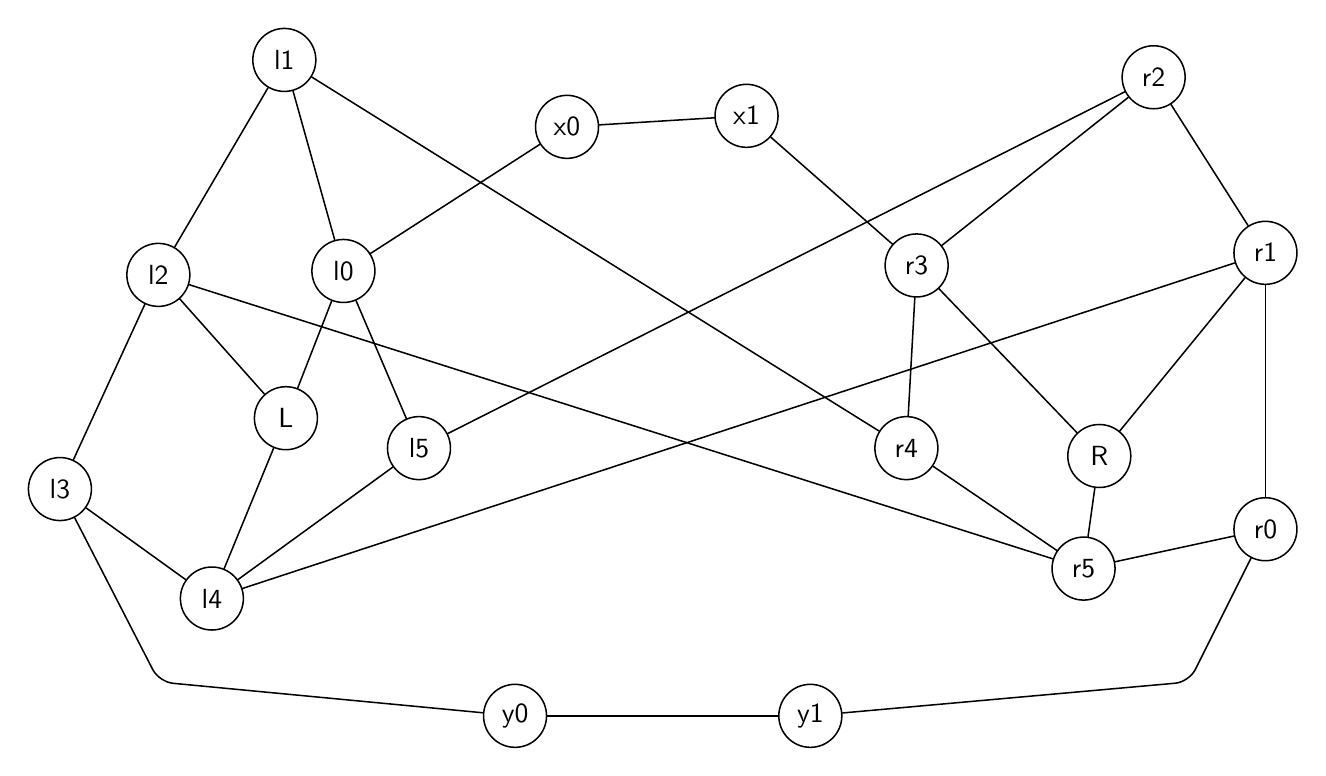
\begin{tikzpicture}[x=1cm,y=1cm]
\tikzset{
  graphnode/.style={circle,draw=black,line width=0.55pt,minimum size=8mm,inner sep=1pt,font=\sffamily},
  graphedge/.style={draw=black,line width=0.55pt,line cap=round,line join=round},
  directed/.style={graphedge,-{Stealth[length=2.4mm,width=2.0mm]}},
  undirected/.style={graphedge}
}
\node[graphnode] (n_L) at (-0.80,-0.69) {L};
\node[graphnode] (n_l0) at (-0.07,1.18) {l0};
\node[graphnode] (n_l1) at (-0.82,3.86) {l1};
\node[graphnode] (n_l2) at (-2.42,1.13) {l2};
\node[graphnode] (n_l3) at (-3.67,-1.59) {l3};
\node[graphnode] (n_l4) at (-1.74,-2.98) {l4};
\node[graphnode] (n_l5) at (0.89,-1.07) {l5};
\node[graphnode] (n_R) at (9.53,-1.17) {R};
\node[graphnode] (n_r0) at (11.64,-2.10) {r0};
\node[graphnode] (n_r1) at (11.64,1.41) {r1};
\node[graphnode] (n_r2) at (10.22,3.64) {r2};
\node[graphnode] (n_r3) at (7.21,1.25) {r3};
\node[graphnode] (n_r4) at (7.08,-1.07) {r4};
\node[graphnode] (n_r5) at (9.33,-2.60) {r5};
\node[graphnode] (n_x0) at (2.77,3.01) {x0};
\node[graphnode] (n_x1) at (5.05,3.15) {x1};
\node[graphnode] (n_y0) at (2.11,-4.47) {y0};
\node[graphnode] (n_y1) at (5.86,-4.47) {y1};
\draw[undirected] (n_l0) -- (n_l1);
\draw[undirected] (n_l1) -- (n_l2);
\draw[undirected] (n_l2) -- (n_l3);
\draw[undirected] (n_l3) -- (n_l4);
\draw[undirected] (n_l4) -- (n_l5);
\draw[undirected] (n_l5) -- (n_l0);
\draw[undirected] (n_L) -- (n_l0);
\draw[undirected] (n_L) -- (n_l2);
\draw[undirected] (n_L) -- (n_l4);
\draw[undirected] (n_r0) -- (n_r1);
\draw[undirected] (n_r1) -- (n_r2);
\draw[undirected] (n_r2) -- (n_r3);
\draw[undirected] (n_r3) -- (n_r4);
\draw[undirected] (n_r4) -- (n_r5);
\draw[undirected] (n_r5) -- (n_r0);
\draw[undirected] (n_R) -- (n_r1);
\draw[undirected] (n_R) -- (n_r3);
\draw[undirected] (n_R) -- (n_r5);
\draw[undirected] (n_l0) -- (n_x0);
\draw[undirected] (n_x0) -- (n_x1);
\draw[undirected] (n_x1) -- (n_r3);
\draw[undirected,rounded corners=5pt] (n_l3) -- (-2.41,-4.04) -- (n_y0);
\draw[undirected] (n_y0) -- (n_y1);
\draw[undirected,rounded corners=5pt] (n_y1) -- (10.67,-4.04) -- (n_r0);
\draw[undirected] (n_l1) -- (n_r4);
\draw[undirected] (n_l2) -- (n_r5);
\draw[undirected] (n_l4) -- (n_r1);
\draw[undirected] (n_l5) -- (n_r2);
\end{tikzpicture}
\end{document}
